\subsubsection{Caso d'uso UC8.1.3.1: Creazione domanda vero/falso}
	\label{UC8.1.3.1}
	\begin{figure}[h]
		\centering
			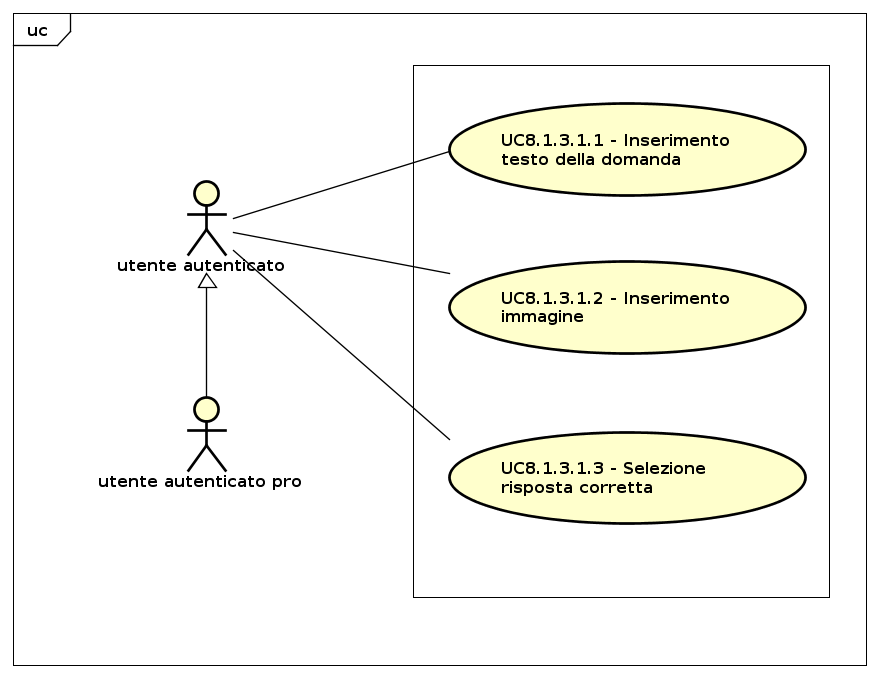
\includegraphics[scale=0.45,keepaspectratio]{UML/UC8_1_3_1.png}
		\caption{UC8.1.3.1: Creazione domanda vero/falso}
	\end{figure}
	\FloatBarrier
	\begin{itemize}
		\item
			\textbf{Attori}: utente autenticato, utente autenticato pro;
		\item		
			\textbf{Descrizione}: l'attore può creare domande vero/falso;
		\item
			\textbf{Precondizione}: l'attore ha selezionato la seguente funzionalità; 
		\item
			\textbf{Postcondizione}: l'attore ha creato una domanda vero/falso;
		\item
			\textbf{Scenario principale}:
	       		\begin{enumerate}
	       			\item
	       			L'attore può compilare il campo dati destinato alla scrittura del testo della domanda (UC8.1.3.1.1)
	       			\item
	       			L'attore può inserire un'immagine relativa al testo della domanda (UC8.1.3.1.2)
					\item
					L'attore può indicare la risposta corretta tramite uno strumento di selezione (UC8.1.3.1.3).
	 			\end{enumerate}
	\end{itemize}

\subsubsection{Caso d'uso UC8.1.3.1.1: Inserimento testo della domanda}
	\begin{itemize}
		\item
			\textbf{Attori}: utente autenticato, utente autenticato pro;
		\item		
			\textbf{Descrizione}: l'attore può inserire il testo della domanda;
		\item
			\textbf{Precondizione}: l'attore ha selezionato la modalità di creazione di una domanda vero/falso; 
		\item
			\textbf{Postcondizione}: l'attore ha inserito il testo della domanda;
		\item
			\textbf{Scenario principale}: l'attore inserisce il testo della domanda. 
	 			
	\end{itemize}
	
\subsubsection{Caso d'uso UC8.1.3.1.2: Inserimento immagine}
	\label{UC8.1.3.1.2}
	\begin{figure}[h]
		\centering
			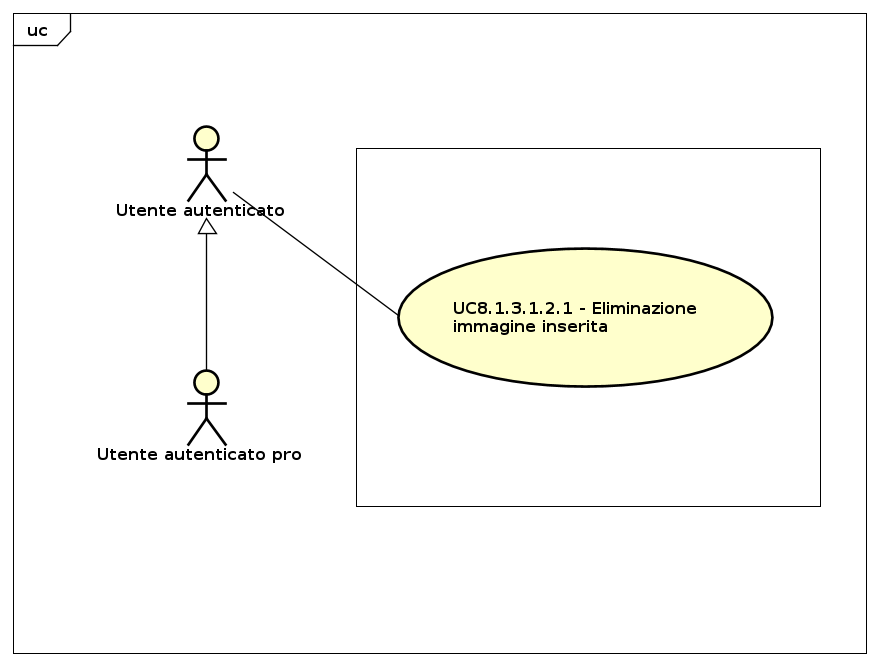
\includegraphics[scale=0.45,keepaspectratio]{UML/UC8_1_3_1_2.png}
		\caption{UC8.1.3.1.2: Inserimento immagine}
	\end{figure}
	\FloatBarrier
	\begin{itemize}
		\item
			\textbf{Attori}: utente autenticato, utente autenticato pro;
		\item		
			\textbf{Descrizione}: l'attore può inserire un'immagine relativa al testo della domanda;
		\item
			\textbf{Precondizione}: l'attore ha selezionato la modalità di creazione di una domanda vero/falso; 
		\item
			\textbf{Postcondizione}: l'attore ha inserito l'immagine;
		\item
			\textbf{Scenario principale}: 
			\begin{enumerate}
				\item
					L'attore può eliminare l'immagine inserita (UC8.1.3.1.2.1).	
			\end{enumerate}						
	\end{itemize}
	\subsubsection{Caso d'uso UC8.1.3.1.2.1: Eliminazione immagine inserita}
		\begin{itemize}
		\item
			\textbf{Attori}: utente autenticato, utente autenticato pro;
		\item		
			\textbf{Descrizione}: l'attore può eliminare l'immagine inserita relativa al testo della domanda;
		\item
			\textbf{Precondizione}: il sistema presenta all'attore lo strumento per compiere questa operazione;
		\item
			\textbf{Postcondizione}: l'immagine inserita è stata eliminata;
		\item
			\textbf{Scenario principale}: l'attore elimina l'immagine inserita.				
		\end{itemize}

\subsubsection{Caso d'uso UC8.1.3.1.3: Selezione risposta corretta}
	\begin{itemize}
		\item
			\textbf{Attori}: utente autenticato, utente autenticato pro;
		\item		
			\textbf{Descrizione}: l'attore può indicare la risposta corretta tramite uno strumento di selezione;
		\item
			\textbf{Precondizione}: l'attore ha selezionato la modalità di creazione di una domanda vero/falso; 
		\item
			\textbf{Postcondizione}: l'attore ha selezionato la risposta corretta;
		\item
			\textbf{Scenario principale}: l'attore indica la risposta corretta tramite uno strumento di selezione. 
	 			
	\end{itemize}
	

	
